\documentclass[10pt]{article}
\usepackage[letterpaper,margin=0.82in]{geometry}
\usepackage[T1]{fontenc}
\usepackage[utf8]{inputenc}
\usepackage{lmodern}
\usepackage{microtype}
\usepackage{amsmath,amssymb,amsthm,mathtools,bm}
\usepackage{booktabs,tabularx,array,multirow}
\usepackage{graphicx}
\usepackage{caption}
\usepackage{subcaption}
\usepackage{enumitem}
\usepackage{hyperref}
\usepackage{fancyhdr}
\usepackage{siunitx}
\usepackage{float}
\usepackage[section]{placeins}
\usepackage{url}
\usepackage{xcolor}
\usepackage{longtable}
\usepackage{threeparttable}
\usepackage{etoolbox}

\graphicspath{{figures/}}
\setlength{\parindent}{1.25em}
\setlength{\parskip}{0pt}
\setlength{\emergencystretch}{2em}
\setlength{\textfloatsep}{8pt plus 2pt minus 2pt}
\setlength{\floatsep}{7pt plus 2pt minus 2pt}
\setlength{\intextsep}{7pt plus 2pt minus 2pt}
\captionsetup{font=small,labelfont=bf}
\renewcommand{\arraystretch}{1.12}
\newcolumntype{Y}{>{\raggedright\arraybackslash}X}
\newcolumntype{R}{>{\raggedleft\arraybackslash}p{1.55cm}}
\newtheorem{proposition}{Proposition}
\newtheorem{theorem}{Theorem}
\newtheorem{corollary}{Corollary}
\newtheorem{lemma}{Lemma}
\newtheorem{example}{Example}
\theoremstyle{remark}
\newtheorem{remark}{Remark}
\newcommand{\E}{\mathbb{E}}
\newcommand{\Var}{\operatorname{Var}}
\newcommand{\Cov}{\operatorname{Cov}}
\newcommand{\AsVar}{\operatorname{AsVar}}
\newcommand{\rESS}{\mathrm{rESS}}
\newcommand{\pWIS}{\mathrm{pWIS}}
\newcommand{\ind}{\mathbf{1}}
\newcommand{\dd}{\,\mathrm{d}}
% Auto-generated from frozen output tables. Do not edit numbers by hand.
\newcommand{\SvLowRess}{0.138}
\newcommand{\SvMedRess}{0.212}
\newcommand{\SvHighRess}{0.974}
\newcommand{\SvOldRess}{0.142}
\newcommand{\SvRecentRess}{0.965}
\newcommand{\SvMatchedRessCount}{6/6}
\newcommand{\SvOldMAE}{0.00856}
\newcommand{\SvRecentMAE}{0.00230}
\newcommand{\SvMAEReduction}{73.1\%}
\newcommand{\SvMatchedMAECount}{5/6}
\newcommand{\SvOldRMSE}{0.01030}
\newcommand{\SvRecentRMSE}{0.00254}
\newcommand{\SvRMSEReduction}{75.3\%}
\newcommand{\SvGateAcceptOne}{100.0\%}
\newcommand{\SvGateFAOne}{25.00\%}
\newcommand{\SvGateAcceptTwo}{100.0\%}
\newcommand{\SvGateFATwo}{4.17\%}
\newcommand{\SvGateAcceptFive}{100.0\%}
\newcommand{\SvGateFAFive}{0.00\%}
\newcommand{\SvISMAE}{0.004996}
\newcommand{\SvISRMSE}{0.006262}
\newcommand{\SvPWISMAE}{0.007102}
\newcommand{\SvPWISRMSE}{0.009266}
\newcommand{\GsmOldRMSE}{0.00736}
\newcommand{\GsmRecentRMSE}{0.00214}
\newcommand{\AlphaDevPairs}{45}
\newcommand{\AlphaDevOldRess}{0.125}
\newcommand{\AlphaDevRecentRess}{0.957}
\newcommand{\AlphaDevOldAlpha}{0.04850}
\newcommand{\AlphaDevRecentAlpha}{0.05094}
\newcommand{\AlphaDevAlphaFav}{18/45}
\newcommand{\AlphaDevOldA}{0.04615}
\newcommand{\AlphaDevRecentA}{0.04834}
\newcommand{\AlphaDevMtwoFav}{45/45}
\newcommand{\AlphaDevMeanMtwoRatio}{0.0748}
\newcommand{\AlphaDevGeoMtwoRatio}{0.0735}
\newcommand{\AlphaDevVMin}{0.04260}
\newcommand{\AlphaDevVMax}{0.05821}
\newcommand{\AlphaTestPairs}{9}
\newcommand{\AlphaTestOldRess}{0.127}
\newcommand{\AlphaTestRecentRess}{0.959}
\newcommand{\AlphaTestOldAlpha}{0.04016}
\newcommand{\AlphaTestRecentAlpha}{0.04589}
\newcommand{\AlphaTestAlphaFav}{2/9}
\newcommand{\AlphaTestOldA}{0.03857}
\newcommand{\AlphaTestRecentA}{0.04378}
\newcommand{\AlphaTestMtwoFav}{9/9}
\newcommand{\AlphaTestMeanMtwoRatio}{0.0793}
\newcommand{\AlphaTestGeoMtwoRatio}{0.0661}
\newcommand{\AlphaTestVMin}{0.04085}
\newcommand{\AlphaTestVMax}{0.05032}


\pagestyle{fancy}
\fancyhf{}
\fancyhead[L]{\small Historical GRPO Trace Reuse}
\fancyhead[R]{\small S. Li}
\fancyfoot[C]{\thepage}
\renewcommand{\headrulewidth}{0pt}
\hypersetup{colorlinks=true,linkcolor=black,citecolor=black,urlcolor=black,pdfauthor={Shenggang Li},pdftitle={When Can Historical GRPO Reasoning Traces Be Reused?}}

\title{\textbf{When Can Historical GRPO Reasoning Traces Be Reused?}\\[0.25em]
\large Off-Policy Evaluation and Trace Refresh under Policy Drift}
\author{Shenggang Li\\Independent Researcher\\\texttt{datalev@gmail.com}}
\date{}

\begin{document}
\maketitle
\vspace{-1.4em}

\begin{abstract}
Reinforcement learning for language models produces large collections of reasoning traces while the policy continues to change. Reusing these traces to evaluate later checkpoints can save substantial sampling cost, but it creates an off-policy evaluation problem as sequence likelihood ratios become increasingly concentrated under policy drift. We study this problem along three GRPO training paths, treating earlier checkpoints as behavior policies and later checkpoints as targets. Historical completions are rescored with exact sequence likelihood ratios, and prompt-normalized weighted importance sampling is evaluated against independent finite on-policy Monte Carlo references.

Building on standard self-normalized importance-sampling theory, we separate the leading prompt-WIS risk into second-moment overlap and reward-residual components. For autoregressive trajectories, a prefix second-moment recursion shows how sequence-level R\'enyi-2 mismatch accumulates through tokenwise conditional mismatch under a squared-weight tilted prefix law. For binary correctness rewards, the residual component identifies how squared-weight concentration is allocated between correct and incorrect trajectories, and a shared-reference identity clarifies how finite reference noise enters matched comparisons. On the untouched GSM8K test set, matched replacement of the stale log by a recent behavior log increases mean pair-level median rESS from 0.127 to 0.959 in all 9 comparisons and reduces mean absolute reference discrepancy from 0.00587 to 0.00164, with improvement in 8 of 9 cases. A separately frozen SVAMP stress test, performed without pair reselection or gate refitting, preserves the predeclared overlap ordering and the refresh effect: median rESS rises from \SvOldRess\ to \SvRecentRess\ in \SvMatchedRessCount\ matched comparisons and mean absolute reference discrepancy falls from \SvOldMAE\ to \SvRecentMAE\ in \SvMatchedMAECount. In contrast, the frozen scalar rESS gate accepts every external case and false-accepts \SvGateFAOne\ at the 1\% tolerance. The evidence therefore supports overlap-aware trace refresh, but not a universal one-dimensional reuse certificate.
\end{abstract}

\noindent\textbf{Keywords:} off-policy evaluation; GRPO; reasoning traces; importance sampling; effective sample size; policy drift; data reuse; external validation.

\section{Introduction}
Reinforcement learning for language models creates evaluation data as a by-product of optimization. A GRPO update starts from a batch of prompts, samples several completions, assigns rewards, and changes the policy. Repeating this process leaves a sequence of checkpoints together with a growing archive of expensive reasoning traces. Regenerating comparable traces at every later checkpoint repeats inference and reward computation that the training run has already paid for once. The practical question is therefore not merely whether old traces can be stored, but when they remain statistically defensible as evidence for a changed policy.

If the policy were fixed, previously sampled completions would still be draws from the policy being evaluated. Once the policy changes, reuse becomes an off-policy evaluation (OPE) problem. A completion $y$ sampled from a behavior checkpoint $\mu_b(\cdot\mid x)$ may receive a very different probability under a later target checkpoint $\pi_e(\cdot\mid x)$. For an autoregressive model, the likelihood of the observed token path can be recomputed under both checkpoints, so the change-of-measure ratio is available. The difficulty is statistical rather than algebraic: small token-level differences multiply across a long sequence, concentrating importance weights and shrinking the effective evidence in a nominally large trace set. This is the familiar curse of horizon in importance sampling~\cite{liu2020horizon}, expressed here through language-model reasoning trajectories.

We study this aging of historical evidence in two complementary ways. A fixed-log frontier holds the behavior checkpoint at step 0 while the target moves along the GRPO training path. A matched-refresh design then fixes the target checkpoint and compares the same target using either the stale step-0 log or a more recent behavior log. In the matched comparison, the target policy, prompt set, reward definition, and on-policy reference do not change; only the source of historical evidence changes. Relative effective sample size (rESS) summarizes weight concentration before the reference is read. To test whether this diagnostic can support an operational reuse rule, a simple rESS threshold is calibrated on development data, frozen, and evaluated on a held-out training seed and the official GSM8K test without retuning.

The theoretical analysis deliberately separates established SNIS foundations from trace-reuse-specific consequences. First, a prefix second-moment recursion makes the autoregressive horizon mechanism explicit: tokenwise conditional mismatch is accumulated under a squared-weight tilted prefix law, so earlier likelihood-ratio concentration changes which later prefixes dominate second-moment risk. Second, the standard SNIS asymptotic variance factors into a second-moment overlap term and a reward-residual term; for binary correctness rewards, the latter can be written through the squared-weight tilted mass on correct trajectories, yielding a problem-specific two-channel refresh comparison. Third, because the old- and recent-log estimates use the same independently generated on-policy reference, reference noise contributes the same additive term to their expected squared discrepancies and cancels in the expected old-versus-recent comparison. These results describe temporal accumulation, reward allocation, and measurement noise without claiming a new generic theory of SNIS.

The evidence architecture is intentionally staged. GSM8K development data establish the dense frontier and calibrate the diagnostic gate; one training seed is held out from gate fitting; the official GSM8K test provides an untouched in-domain evaluation; and a separately frozen SVAMP experiment then asks whether the same trace-reuse structure survives a prompt-distribution shift. The SVAMP pair registry, estimator, scoring contract, and gate are frozen before any SVAMP OPE or reference outcome is inspected. This distinction matters: the external experiment is a falsification test of a previously defined reuse protocol, not a second round of tuning.

The resulting picture is sharper than a simple claim that ``fresh data are better.'' Fixed historical logs lose overlap along all three training paths, but checkpoint age alone does not determine realized reference discrepancy. Replacing stale logs with recent logs restores high overlap in every matched GSM8K test comparison and in every matched SVAMP comparison. Yet a scalar rESS gate remains nonselective on both the GSM8K test and SVAMP. A post-hoc mechanism analysis, kept explicitly exploratory, further shows that the reward-stratum allocation factor often moves in an adverse direction even while the aggregate empirical leading-risk proxy improves. Thus overlap restoration is powerful but not a complete finite-sample certificate.

The paper therefore separates four questions: how historical support ages; whether matched refresh repairs support for a fixed target; how overlap and reward-stratum allocation jointly enter leading risk; and whether a one-dimensional overlap diagnostic is sufficient for reuse decisions. The answer to the first three is strongly structured in this controlled setting; the answer to the fourth is negative.

\section{Related Work}
\paragraph{GRPO and reasoning-policy evolution.}
GRPO was introduced in the DeepSeekMath line of work as a group-relative policy-optimization method for mathematical reasoning~\cite{shao2024deepseekmath}; later reasoning systems emphasized reinforcement learning over sampled solution traces at larger scale~\cite{deepseek2025r1}. These methods naturally create checkpointed policy paths and repeated completion samples. We use that training process as an empirical source of behavior and target policies rather than proposing a modification to the GRPO objective.

\paragraph{Off-policy evaluation and support.}
Importance-weighted and self-normalized OPE are well established~\cite{dudik2011dr,jiang2016dr,swaminathan2015selfnorm}, while high-confidence extensions study how limited support affects downstream policy decisions~\cite{thomas2015hcpi,kuzborskij2021confident}. Non-asymptotic SNIS theory connects approximation error to second moments of importance weights~\cite{agapiou2017}; work on effective sample size emphasizes that normalized-weight ESS is useful as a diagnostic but is not, in general, a complete estimator-specific uncertainty measure~\cite{martino2017ess,elvira2022ess}. Bias-reduction methods for self-normalized estimators further illustrate the dispersion--bias trade-off~\cite{cardoso2022brsnis}. We use these results as foundations rather than as claims of estimator novelty.

\paragraph{Stale rollouts for training versus historical traces for evaluation.}
Recent LLM-RL work reuses stale or replayed rollouts to improve training efficiency. RePO retrieves off-policy samples from a replay buffer~\cite{li2025repo}; off-policy variants of GRPO explicitly modify the optimization objective to accommodate older samples~\cite{mroueh2025grpo}; and Mu-GRPO studies substantially larger rollout staleness while preserving training stability~\cite{tian2026mugrpo}. Those works ask whether stale trajectories can still produce useful policy updates. Our question is different: the target checkpoint is fixed, no gradient update is performed, and historical trajectories are used only to estimate that target's policy value. An importance ratio acceptable inside a clipped training objective need not be the exact change-of-measure weight required for trajectory OPE.

\paragraph{Off-policy language-model evaluation.}
Logged language-model feedback has already been used for OPE~\cite{bhargava2024ope}. Other recent LLM-RL methods use sequence-level importance ratios, including Group Sequence Policy Optimization and tapered off-policy REINFORCE~\cite{zheng2025gspo,leroux2025topr}; off-policy-corrected reward modeling addresses a related distribution-shift problem~\cite{ackermann2025ocrm}. The present study instead follows the same evolving GRPO policy through checkpoints and asks how historical reasoning traces age and recover under refresh at fixed target checkpoints.

\section{Problem Formulation}
Let $x\sim\mathcal D$ be a prompt, $y=(a_1,\ldots,a_T)$ a generated completion, and $r(x,y)\in[0,1]$ the evaluation reward. In the GSM8K and SVAMP experiments the primary reward is correctness of the extracted final answer. A checkpoint at training step $b$ defines a behavior policy $\mu_b$, while a later checkpoint $e$ defines the target policy $\pi_e$. The theoretical results assume the usual support condition $\pi_e(\cdot\mid x)\ll\mu_b(\cdot\mid x)$. In the implemented softmax policies, every logged token on every trajectory used for rescoring has strictly positive probability under both relevant checkpoints, so evaluated sequence ratios are finite on the observed paths.

For prompt $x_i$, a historical log collected at $b$ contains $K$ completions,
\begin{equation}
\mathcal L_{b,i}=\{(y_{ij},r_{ij},\log\mu_b(y_{ij}\mid x_i))\}_{j=1}^{K}.
\end{equation}
The sequence importance ratio for target checkpoint $e$ is
\begin{equation}
W_{ij}^{(b\to e)}=\frac{\pi_e(y_{ij}\mid x_i)}{\mu_b(y_{ij}\mid x_i)},\qquad
\log W_{ij}^{(b\to e)}=\log\pi_e(y_{ij}\mid x_i)-\log\mu_b(y_{ij}\mid x_i).
\end{equation}
The population policy value is
\begin{equation}
V_{\mathcal D}(\pi_e)=\E_{x\sim\mathcal D}\E_{y\sim\pi_e(\cdot\mid x)}[r(x,y)].
\end{equation}
The experiments condition on a frozen prompt set $x_1,\ldots,x_n$ and target
\begin{equation}
V_n(\pi_e)=\frac1n\sum_{i=1}^{n}v_i(\pi_e),\qquad
v_i(\pi_e)=\E_{y\sim\pi_e(\cdot\mid x_i)}[r(x_i,y)].
\end{equation}
Each target checkpoint receives an independent on-policy Monte Carlo estimate of this same $V_n(\pi_e)$. The reference is a finite-sample estimate rather than exact truth. Throughout the empirical sections, deviations from this finite reference are called \emph{reference discrepancies}; the term \emph{error} is reserved for deviation from $V_n$ in theoretical statements.

For each prompt, the primary estimator is prompt-normalized weighted importance sampling,
\begin{equation}
\widehat v_i^{\pWIS}=\frac{\sum_{j=1}^{K}W_{ij}r_{ij}}{\sum_{j=1}^{K}W_{ij}},\qquad
\widehat V^{\pWIS}=\frac1n\sum_{i=1}^{n}\widehat v_i^{\pWIS}.
\end{equation}
Prompt normalization matches the finite-prompt estimand: every evaluation prompt receives equal outer weight, while its historical completions are reweighted internally. Ordinary trajectory IS is retained as a secondary estimator benchmark.

For the $K$ historical completions of prompt $i$, empirical relative effective sample size is
\begin{equation}
\widehat{\rESS}_i=\frac{\left(\sum_{j=1}^{K}W_{ij}\right)^2}{K\sum_{j=1}^{K}W_{ij}^2}.
\end{equation}
The primary pair-level overlap diagnostic is the median of this finite-$K$ quantity across prompts. It should not be identified with the population quantity introduced next; with $K=16$, sampling variation in empirical rESS is itself part of the diagnostic uncertainty.

\section{Theory of Historical-Trace Reuse}
For a fixed prompt, suppress $x$ from the notation. Let $Y\sim\mu$, define $W(Y)=\pi(Y)/\mu(Y)$, assume $\pi\ll\mu$, and suppose $\kappa_2:=\E_\mu[W^2]<\infty$. The first two results are standard importance-sampling facts. The later decomposition and refresh consequences are specialized to checkpoint-indexed trace reuse.

\subsection{Second-moment overlap}
\begin{proposition}[Standard second-moment identity]
Under the assumptions above, $\E_\mu[W]=1$ and
\begin{equation}
D_2(\pi\Vert\mu)=\log\kappa_2,\qquad \rESS_\infty=\frac1{\kappa_2}=e^{-D_2(\pi\Vert\mu)}.
\end{equation}
If $W_1,\ldots,W_K$ are i.i.d. under $\mu$, empirical rESS converges almost surely to $\rESS_\infty$.
\end{proposition}
We use
\begin{equation}
K_{\mathrm{eff}}^{(2)}=\frac{K}{\kappa_2}=Ke^{-D_2(\pi\Vert\mu)}
\end{equation}
as a second-moment effective trace count. It is a population coordinate, not a literal finite-sample sample size. For ordinary IS and $0\le R\le1$,
\begin{equation}
\Var_\mu\!\left(\frac1K\sum_{j=1}^{K}W_jR_j\right)\le \frac{\kappa_2}{K}=\frac1{K_{\mathrm{eff}}^{(2)}}.
\end{equation}

\subsection{Finite-sample SNIS foundation}
\begin{theorem}[SNIS MSE bound for bounded rewards; consequence of Agapiou et al.]
Let $Y_1,\ldots,Y_K\stackrel{\mathrm{iid}}{\sim}\mu$, $R_j=r(Y_j)\in[0,1]$, $W_j=\pi(Y_j)/\mu(Y_j)$, $v=\E_\pi[R]$, and $\widehat v=\sum_jW_jR_j/\sum_jW_j$. Then
\begin{equation}
\E_\mu[(\widehat v-v)^2]\le \min\!\left\{1,\frac{\kappa_2}{K}\right\},\qquad
|\E_\mu[\widehat v]-v|\le \min\!\left\{1,\frac{6\kappa_2}{K}\right\}.
\end{equation}
\end{theorem}
The constants follow by applying the standard Agapiou et al. bound~\cite{agapiou2017} to $\phi=2R-1$, for which $|\phi|\le1$. The result remains deliberately conservative: it depends on $\kappa_2$ alone and does not distinguish where high weights fall relative to reward residuals.

\subsection{Overlap--reward-residual decomposition}
Define the squared-weight tilted probability law
\begin{equation}
\nu_2(\dd y):=\frac{W(y)^2}{\kappa_2}\mu(\dd y),
\end{equation}
and the reward-residual factor
\begin{equation}
A_\mu:=\E_{\nu_2}[(R-v)^2]=\frac{\E_\mu[W^2(R-v)^2]}{\kappa_2}.
\end{equation}
Because $R\in[0,1]$, $0\le A_\mu\le1$.

\begin{proposition}[Overlap--reward-residual decomposition]
Under the assumptions of Theorem 1,
\begin{equation}
\sqrt K(\widehat v-v)\Rightarrow N(0,m_2),\qquad m_2:=\E_\mu[W^2(R-v)^2].
\end{equation}
Moreover,
\begin{equation}
m_2=\Var_\mu\{W(R-v)\}=\kappa_2A_\mu,\qquad \frac{m_2}{K}=\frac{A_\mu}{K_{\mathrm{eff}}^{(2)}}.
\end{equation}
\end{proposition}
Thus $\kappa_2$ measures second-moment support mismatch, whereas $A_\mu$ measures the squared reward residual under the law that emphasizes trajectories with large squared importance weight. This is an interpretation of the standard SNIS asymptotic variance, not a new generic SNIS central-limit theorem.

\subsection{Fixed-target refresh and the aggregate estimator}
Consider the same target policy $\pi_e$ evaluated from an old log $\mu_o$ and a recent log $\mu_r$. Let $(\kappa_o,A_o)$ and $(\kappa_r,A_r)$ denote the corresponding quantities.

\begin{corollary}[Fixed-target refresh risk ratio]
If $A_o>0$ and $A_r>0$, then
\begin{equation}
\frac{m_{2,r}}{m_{2,o}}=\frac{\kappa_rA_r}{\kappa_oA_o}
=\exp\{D_2(\pi_e\Vert\mu_r)-D_2(\pi_e\Vert\mu_o)\}\frac{A_r}{A_o}.
\end{equation}
Consequently,
\begin{equation}
D_2(\pi_e\Vert\mu_o)-D_2(\pi_e\Vert\mu_r)>\log\frac{A_r}{A_o}
\quad\Longrightarrow\quad m_{2,r}<m_{2,o}.
\end{equation}
\end{corollary}
The condition separates two mechanisms that a comparison based on $\kappa_2$ alone cannot distinguish: refresh can improve overlap while an adverse change in reward-residual alignment offsets part of that gain. It concerns leading risk, not a deterministic ordering of realized Monte Carlo discrepancies.

\begin{corollary}[Prompt-grouped leading variance coefficient]
Condition on a fixed set of $n$ prompts and suppose completion groups are independent across prompts. Let $m_{2,i}=\kappa_{2,i}A_i$ be the promptwise coefficient in Proposition 2. For fixed $n$ and $K\to\infty$,
\begin{equation}
\sqrt K\left(\widehat V^{\pWIS}-V_n\right)\Rightarrow
N\!\left(0,\frac1{n^2}\sum_{i=1}^{n}m_{2,i}\right).
\end{equation}
Equivalently,
\begin{equation}
\AsVar(\widehat V^{\pWIS}\mid x_{1:n})=\frac1{n^2K}\sum_{i=1}^{n}m_{2,i}=\frac{\bar m_2}{nK},\qquad
\bar m_2:=\frac1n\sum_{i=1}^{n}m_{2,i}.
\end{equation}
\end{corollary}
This form makes the experimental sampling geometry explicit. The leading coefficient depends on the promptwise $\kappa_{2,i}A_i$, not on median empirical rESS alone.

\subsection{Prefix second-moment recursion for autoregressive traces}
The sequence ratio is a product of tokenwise ratios. To place variable-length completions on one filtration, fix the generation cap $T_{\max}$ and, after the first EOS token, extend both policies by the same absorbing transition. Hence subsequent likelihood ratios equal one. Let $H_{t-1}$ denote the padded prefix before token $t$, and define
\begin{equation}
w_t(a\mid h):=\frac{\pi_t(a\mid h)}{\mu_t(a\mid h)},\qquad
W_t:=\prod_{s=1}^{t}w_s(A_s\mid H_{s-1}),\qquad W_0:=1.
\end{equation}
Let
\begin{equation}
\kappa_{2,t}:=\E_\mu[W_t^2],\qquad
c_t(h):=\E_{A_t\sim\mu_t(\cdot\mid h)}[w_t(A_t\mid h)^2]=\exp\{d_{2,t}(h)\},
\end{equation}
where $d_{2,t}(h):=D_2(\pi_t(\cdot\mid h)\Vert\mu_t(\cdot\mid h))$. For $\kappa_{2,t-1}>0$, define the squared-weight tilted prefix law
\begin{equation}
\nu_{t-1}^{(2)}(\dd h):=\frac{W_{t-1}(h)^2}{\kappa_{2,t-1}}\mu_{1:t-1}(\dd h).
\end{equation}

\begin{proposition}[Prefix second-moment recursion]
Under tokenwise absolute continuity and finite second moments,
\begin{equation}
\kappa_{2,t}=\kappa_{2,t-1}\E_{\nu_{t-1}^{(2)}}[c_t(H_{t-1})].
\end{equation}
Consequently,
\begin{equation}
D_2(\pi_{1:T_{\max}}\Vert\mu_{1:T_{\max}})
=\sum_{t=1}^{T_{\max}}\log\E_{\nu_{t-1}^{(2)}}[\exp\{d_{2,t}(H_{t-1})\}],
\end{equation}
and
\begin{equation}
D_2(\pi_{1:T_{\max}}\Vert\mu_{1:T_{\max}})
\ge \sum_{t=1}^{T_{\max}}\E_{\nu_{t-1}^{(2)}}[d_{2,t}(H_{t-1})].
\end{equation}
Moreover, $\kappa_{2,t}$ is nondecreasing in $t$, the corresponding population prefix rESS $1/\kappa_{2,t}$ is nonincreasing, and
\begin{equation}
\E_{\nu_{t-1}^{(2)}}[c_t]-\E_{\mu_{1:t-1}}[c_t]
=\frac{\Cov_{\mu_{1:t-1}}(W_{t-1}^2,c_t)}{\kappa_{2,t-1}}.
\end{equation}
\end{proposition}
The recursion is an exact tower-property identity, not a Shannon-style additive chain rule for R\'enyi divergence. Later conditional mismatch is evaluated under prefixes already tilted by earlier squared likelihood ratios. Early mismatch therefore amplifies later second-moment growth only when later conditional mismatch is positively associated with already high-weight prefixes; there is no universal amplification sign without that covariance condition.

\subsection{Binary correctness and squared-weight strata}
For correctness rewards, $R\in\{0,1\}$. Define
\begin{equation}
\kappa_1:=\E_\mu[W^2\ind\{R=1\}],\qquad
\kappa_0:=\E_\mu[W^2\ind\{R=0\}],\qquad
\alpha_\mu:=\frac{\kappa_1}{\kappa_2}=\nu_2(R=1).
\end{equation}
Thus $\alpha_\mu$ is the fraction of squared-weight mass assigned to correct trajectories under the tilted law.

\begin{proposition}[Binary-stratum risk decomposition]
For binary reward,
\begin{align}
\kappa_2&=\kappa_0+\kappa_1,\\
m_2&=(1-v)^2\kappa_1+v^2\kappa_0\\
&=\kappa_2\{(1-v)^2\alpha_\mu+v^2(1-\alpha_\mu)\}\\
&=\kappa_2\{v^2+(1-2v)\alpha_\mu\}.
\end{align}
For fixed $v$ and $\kappa_2$,
\begin{equation}
\frac{\partial m_2}{\partial\alpha_\mu}=\kappa_2(1-2v).
\end{equation}
\end{proposition}
When $v<1/2$, correct trajectories carry the larger squared residual $(1-v)^2$, so moving squared-weight mass toward the correct stratum increases the leading variance coefficient at fixed $\kappa_2$; when $v>1/2$, the direction reverses.

\begin{corollary}[Binary fixed-target refresh ratio]
For the same binary-reward target with $0<v<1$,
\begin{equation}
\frac{m_{2,r}}{m_{2,o}}=\frac{\kappa_r}{\kappa_o}
\frac{v^2+(1-2v)\alpha_r}{v^2+(1-2v)\alpha_o}.
\end{equation}
\end{corollary}
The target value is identical within a matched comparison. Refresh therefore changes leading risk through two separable channels: total squared-weight concentration and the allocation of squared weight across reward strata.

\subsection{Shared finite references in matched refresh}
The matched comparison uses the same independently generated on-policy reference for the stale- and recent-log estimates.

\begin{lemma}[Shared-reference discrepancy identity]
Condition on the frozen prompt set. Let $\widehat V_s$, $s\in\{o,r\}$, be any logged-data estimator of $V_n$ that is independent of an on-policy reference $\widehat V_{\mathrm{ref}}$, and assume
\begin{equation}
\E[\widehat V_{\mathrm{ref}}\mid x_{1:n}]=V_n.
\end{equation}
Then, for $s\in\{o,r\}$,
\begin{equation}
\E[(\widehat V_s-\widehat V_{\mathrm{ref}})^2\mid x_{1:n}]
=\E[(\widehat V_s-V_n)^2\mid x_{1:n}]+\Var(\widehat V_{\mathrm{ref}}\mid x_{1:n}).
\end{equation}
Consequently,
\begin{equation}
\E[(\widehat V_r-\widehat V_{\mathrm{ref}})^2-(\widehat V_o-\widehat V_{\mathrm{ref}})^2\mid x_{1:n}]
=\operatorname{MSE}(\widehat V_r\mid x_{1:n})-\operatorname{MSE}(\widehat V_o\mid x_{1:n}).
\end{equation}
No independence between $\widehat V_o$ and $\widehat V_r$ is required.
\end{lemma}
Thus finite reference noise increases each expected squared discrepancy by the same additive term and does not change their expected squared-discrepancy ordering. For one realized shared reference, let $\Delta_s=\widehat V_s-V_n$ and $\eta=\widehat V_{\mathrm{ref}}-V_n$. Then
\begin{equation}
(\Delta_r-\eta)^2-(\Delta_o-\eta)^2=(\Delta_r^2-\Delta_o^2)-2\eta(\Delta_r-\Delta_o),
\end{equation}
so a particular reference realization can still reverse the pointwise ordering.

\subsection{Why scalar overlap is not a sufficient risk statistic}
Proposition 4 shows that $\kappa_2$ alone omits reward-stratum allocation. A small finite example makes the point explicit.

\begin{example}[Equal overlap, different OPE risk]
Let the target assign probability $(1/3,1/3,1/3)$ to three trajectories with rewards $(1,0,0)$. Compare $\mu_A=(1/5,2/5,2/5)$ and $\mu_B=(1/2,1/4,1/4)$. Both satisfy $\kappa_2=10/9$, so both have $\rESS_\infty=9/10$. The target value is $v=1/3$, but
\begin{equation}
m_{2,A}=\frac{25}{81},\qquad m_{2,B}=\frac{16}{81}.
\end{equation}
Identical second-moment overlap can therefore coexist with asymptotic variance coefficients differing by a factor $25/16$.
\end{example}

\begin{remark}[Perfect overlap is not an error certificate]
Take $\pi=\mu$, so $W_j\equiv1$ and empirical rESS is identically one. If $R\sim\operatorname{Bernoulli}(1/2)$, pWIS reduces to the sample mean. With probability $2^{1-K}$ all $K$ rewards are zero or all are one, and the absolute estimation error is exactly $1/2$. Even perfect overlap cannot deterministically certify a realized finite-sample tolerance.
\end{remark}

\section{Experimental Design}
Each GRPO run produces a checkpointed language-model policy path together with an archive of sampled reasoning traces. We use that archive in two primary comparisons. The fixed-log frontier holds the behavior log fixed while the target policy advances, measuring how historical evidence ages. The matched-refresh design instead holds the target fixed and replaces a stale behavior log with a more recent one, isolating the effect of refresh. Independent target-policy samples provide the finite reference value in both designs. A frozen rESS rule is evaluated separately as an operational audit of whether an overlap diagnostic can support a reuse decision.

\subsection{GRPO policy paths and trace generation}
GSM8K provides a controlled reasoning environment in which final answers can be verified automatically and target-policy completions can be sampled repeatedly. The original 7,473 training examples are partitioned into 6,000 GRPO-training prompts and 1,473 development prompts; the official 1,319-example test split is isolated until the final test pipeline. The policy is Qwen2.5-0.5B-Instruct with LoRA adaptation. Three independent runs use seeds 20260826, 20260827, and 20260828. Each run lasts 400 update steps, with adapters stored every 20 steps. Training uses four generations per prompt, maximum completion length 128, temperature 1, top-$p$ 1, top-$k$ 0, GRPO $\beta=0.02$, clipping parameter $\epsilon=0.2$, and learning rate $5\times10^{-6}$. The goal is not state-of-the-art GSM8K accuracy; the checkpoint sequence supplies a controlled nonstationary family of related reasoning policies whose historical traces can be audited.

\begin{figure}[H]
\centering
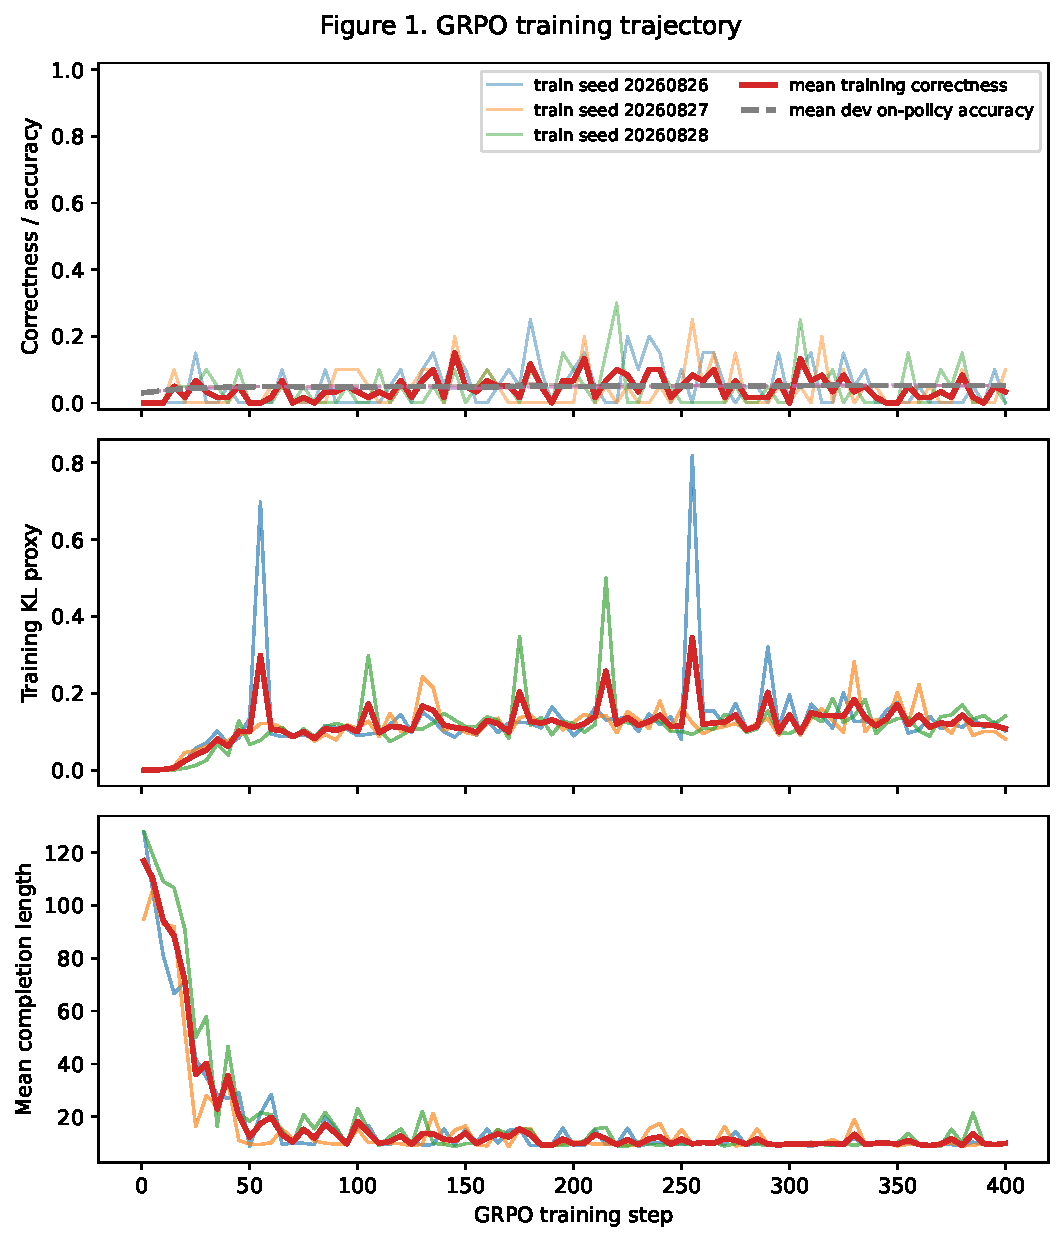
\includegraphics[width=.92\linewidth]{Figure1_training_trajectory.pdf}
\caption{GRPO training paths for the three seeds. The trajectories provide the sequence of behavior and target policies used by the OPE study; checkpoint selection is not based on official-test performance.}
\label{fig:training}
\end{figure}

\subsection{Historical-trace reuse designs}
Each historical behavior log contains $K=16$ completions per prompt. In the fixed-log frontier, the behavior checkpoint is fixed at $b=0$ and the target moves forward along the same training path. Development uses the dense grid $e=20,40,\ldots,400$, giving 60 fixed-log summaries across three seeds. The official test uses eight targets per seed,
\[
e\in\{20,120,160,220,260,300,360,400\},
\]
for 24 fixed cases.

For matched refresh, a fixed target checkpoint is evaluated twice: once from the stale step-0 log and once from a more recent behavior checkpoint. Development uses recent anchors at steps 100, 200, and 300 and yields 45 target-matched comparisons. The official test uses the matched pairs $100\to160$, $200\to260$, and $300\to360$ for each seed, together with the corresponding step-0 comparators, giving nine matched comparisons. The target checkpoint, prompts, reward definition, and on-policy reference are unchanged within each comparison.

\subsection{Rescoring, finite references, and diagnostics}
Formal behavior and target log probabilities are recomputed by symmetric canonical FP32 teacher forcing on the same observed token IDs. Sequence-ratio calculations are performed in log space, and the primary analysis does not clip importance weights. Prompt-WIS is primary because the finite-prompt estimand gives equal outer weight to each prompt; ordinary trajectory IS is retained as a benchmark.

On-policy references are generated independently of the historical logs. The official GSM8K test uses eight target-policy samples per prompt. Conditional on the frozen prompts, if the $L$ correctness draws per prompt are independent Bernoulli samples, the aggregate reference obeys
\begin{equation}
\Var(\widehat V_{\mathrm{ref}}\mid x_{1:n})
=\frac1{n^2}\sum_{i=1}^{n}\frac{v_i(1-v_i)}{L}\le \frac1{4nL}.
\end{equation}
At $n=1319$ and $L=8$, the worst-case standard-error bound is 0.00487. Thus discrepancies of a few $10^{-3}$ should not be read as differences from exact policy value. OPE and reference uncertainty are summarized with 2,000 prompt-cluster bootstrap replicates. Secondary diagnostics include lower-tail rESS, sampled second-order concentration, maximum normalized weight, log-weight moments, a tokenwise KL proxy, completion length, and truncation rate.

\subsection{Frozen gate and chronological separation}
For reference-discrepancy tolerance $\varepsilon\in\{0.01,0.02,0.05\}$, the operational rule is
\begin{equation}
\text{accept reuse}\quad\Longleftrightarrow\quad \operatorname{median}_i\widehat{\rESS}_i\ge\tau_\varepsilon.
\end{equation}
Seeds 20260826 and 20260827 are used for calibration, and seed 20260828 is held out from gate fitting. For each tolerance, the threshold maximizes calibration coverage subject to zero observed false acceptance. Because calibration contains no failures even at 1\%, all three tolerances receive the same threshold $\tau_\varepsilon=0.122393$. It is frozen before held-out, official-test, and SVAMP outcomes are inspected.

\subsection{Frozen external SVAMP stress test and exploratory mechanism analysis}
The external stage transfers the already-defined protocol to a new prompt distribution. A representative registry of eight behavior--target pairs per seed is selected using GSM8K development diagnostics before any SVAMP outcome is generated: three low-overlap fixed pairs, two medium-overlap fixed pairs, and three high-overlap recent-log pairs. The SVAMP evaluation uses 1,000 prompts, $K=16$ historical completions per prompt, the same maximum completion length and sampling parameters, and independent target-policy references with $L=8$ at ordinary targets and $L=32$ at predeclared audit targets. It uses the same symmetric FP32 scoring contract and the frozen GSM8K gate. No GRPO retraining, pair reselection, gate refitting, or new ablation matrix is permitted.

A pre-analysis implementation audit identified a precision-contract mismatch before any SVAMP OPE or reference outcome was generated. The corrected external run uses FP32 policy inference and symmetric FP32 teacher-forced scoring, while the superseded lower-precision artifacts are excluded from results. The amendment and hashes are recorded in the provenance manifest; Appendix~\ref{app:protocol} gives the chronology.

After all confirmatory GSM8K results were observed, we also ran a CPU-only post-hoc mechanism analysis on the already-existing GSM8K matched pairs. For each prompt it computes the squared-weight tilted correctness mass
\begin{equation}
\widehat\alpha_i=\frac{\sum_jW_{ij}^2R_{ij}}{\sum_jW_{ij}^2},
\label{eq:alphahat}
\end{equation}
and the plug-in diagnostic
\begin{equation}
\widehat A_i^{\mathrm{proxy}}(V)=V^2+(1-2V)\widehat\alpha_i,
\qquad
\widehat m_{2,i}^{\mathrm{proxy}}=\widehat\kappa_{2,i}\widehat A_i^{\mathrm{proxy}}(V),
\end{equation}
where $V$ is the matched pair's aggregate finite on-policy reference. These are mechanism diagnostics, not prompt-specific estimates of the latent theoretical $v_i$ terms and not a newly fitted gate. Development is the primary exploratory analysis; the official test is reported only as exploratory replication.

\begin{table}[H]
\centering
\caption{Evidence architecture and analysis status. ``Frozen'' means that the indicated choices were fixed before the corresponding outcome layer was inspected.}
\label{tab:design}
\small
\begin{tabularx}{\linewidth}{@{}p{2.3cm}Y p{2.7cm}p{2.0cm}@{}}
\toprule
Analysis & Comparison & Research role & Cases \\
\midrule
Fixed-log frontier & Step-0 behavior log; later target checkpoint & Controlled aging & 60 dev / 24 test \\
Matched refresh & Step-0 versus recent behavior log; same target & Primary fixed-target contrast & 45 dev / 9 test \\
Frozen rESS gate & Threshold calibrated on development, then fixed & Decision audit & 35 held-out / 33 test \\
SVAMP external stress & Pre-frozen representative pairs and frozen gate & External falsification & 24 cases \\
Post-hoc $\widehat\alpha$ & Existing GSM8K matched pairs only & Exploratory mechanism & 45 dev / 9 test \\
\bottomrule
\end{tabularx}
\end{table}

\section{Results}
\subsection{A fixed historical log loses overlap, but not at a universal step horizon}
Under a fixed step-0 behavior log, sequence overlap deteriorates as the target moves along the GRPO training path. On development data, target checkpoint and median prompt rESS have pooled Spearman correlation $\rho=-0.745$ across 60 prompt-WIS fixed-log summaries; seed-specific correlations are $-0.908$, $-0.854$, and $-0.605$. The official test reproduces the direction on the reduced grid: pooled $\rho=-0.767$ across 24 cases, with seed-specific values $-0.881$, $-0.905$, and $-0.548$.

The decline is concentrated early in the test frontier. Averaging pair-level median rESS across seeds, the value falls from 0.249 at target step 20 to 0.134 at step 120 and then remains between 0.124 and 0.128 through step 400. At a 1\% absolute reference-discrepancy tolerance, every evaluated target is within tolerance for seeds 20260826 and 20260828, whereas seed 20260827 is within tolerance only through step 160 before later evaluated targets exceed it. At 2\% and 5\%, all eight fixed-log test targets for every seed are within tolerance. The between-seed contrast is direct evidence that checkpoint age is not a standalone reuse rule.

\begin{figure}[H]
\centering

\includegraphics[width=.82\linewidth]{Figure2_fixed_reuse_frontier.pdf}
\caption{Official-test fixed-log frontier. Top: absolute prompt-WIS discrepancy from the independent finite on-policy reference. Bottom: median prompt rESS. The same step-0 behavior log is evaluated against later target checkpoints. Overlap falls sharply, while realized reference discrepancy varies substantially by training seed.}
\label{fig:fixed}
\end{figure}

Overlap is much less predictive of realized discrepancy ordering. Median empirical rESS and absolute prompt-WIS reference discrepancy have pooled Spearman correlation $-0.316$ on development data and $-0.098$ on the official test; the three test-seed correlations are $-0.048$, $-0.595$, and $-0.095$. Proposition 2 provides a structural explanation: $\kappa_2$ controls only the overlap factor, while $A_\mu$ and finite-sample randomness can vary independently. Because the plotted quantity is median finite-$K$ rESS rather than population $1/\kappa_2$, diagnostic sampling noise is an additional source of attenuation.

\begin{figure}[H]
\centering
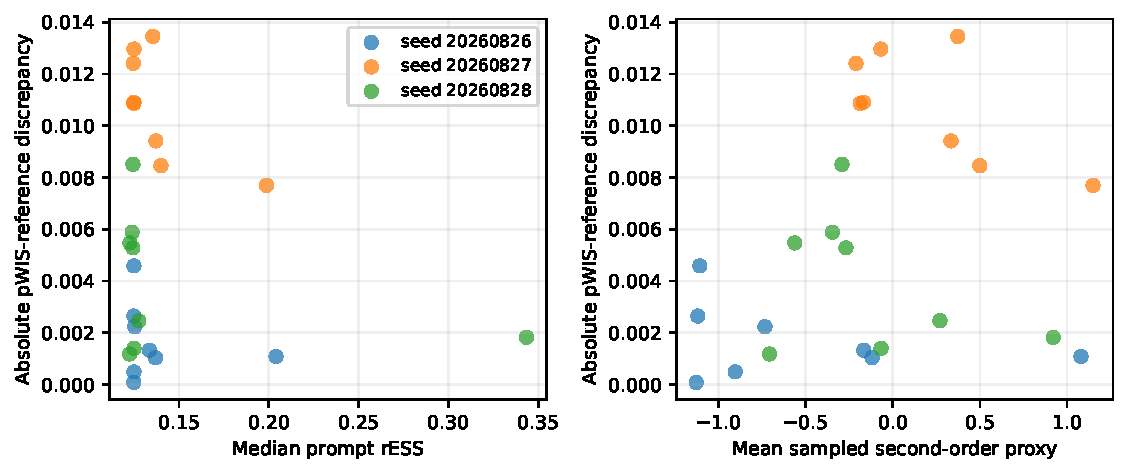
\includegraphics[width=.88\linewidth]{Figure3_overlap_vs_discrepancy.pdf}
\caption{Official-test overlap diagnostics versus absolute prompt-WIS reference discrepancy. Left: median prompt rESS. Right: a sampled second-order concentration proxy derived from observed weights. The latter is an empirical diagnostic, not the population conditional R\'enyi-2 quantity in Section 4.}
\label{fig:diag}
\end{figure}

\subsection{Matched refresh restores effective evidence}
The matched refresh comparison gives the strongest in-domain empirical result. Table~\ref{tab:refresh} places development and official-test outcomes side by side. On development data, a recent log increases median prompt rESS in all 45/45 matched cases: the pair-level mean rises from 0.125 to 0.957. Mean absolute prompt-WIS reference discrepancy falls from 0.005014 to 0.001661, a 66.9\% reduction, with lower discrepancy in 34/45 cases.

The official test reproduces both directions. Mean pair-level median rESS rises from 0.127 under the step-0 log to 0.959 under the recent log, with higher rESS in 9/9 comparisons. Mean absolute reference discrepancy falls from 0.005866 to 0.001642, a 72.0\% reduction, with lower discrepancy in 8/9 comparisons. The mean signed discrepancy moves from $-0.005636$ to $+0.000072$.

\begin{table}[H]
\centering
\caption{Development-to-test replication of the primary trace-reuse findings. rESS entries are means across pair-level median prompt rESS values. Discrepancy quantities use the finite on-policy Monte Carlo reference, not exact policy value.}
\label{tab:refresh}
\small
\begin{tabular}{@{}lrr@{}}
\toprule
Metric & Development & Official test \\
\midrule
Fixed target step vs. median rESS, Spearman $\rho$ & $-0.745$ (60) & $-0.767$ (24) \\
Mean rESS, old $\to$ recent & $0.125\to0.957$ & $0.127\to0.959$ \\
rESS higher after refresh & 45/45 & 9/9 \\
Mean absolute discrepancy, old $\to$ recent & $0.005014\to0.001661$ & $0.005866\to0.001642$ \\
Mean signed discrepancy, old $\to$ recent & $-0.003779\to-0.000272$ & $-0.005636\to+0.000072$ \\
Relative reduction in mean absolute discrepancy & 66.9\% & 72.0\% \\
Lower absolute discrepancy after refresh & 34/45 & 8/9 \\
\bottomrule
\end{tabular}
\end{table}

Figure~\ref{fig:refresh} shows the nine official-test matched cases. Recent-log rESS values are tightly clustered above 0.90, compared with roughly 0.12--0.14 under the stale log. Eight of nine absolute-discrepancy points lie below the equality line; one recent-log estimate is slightly worse. This is consistent with Corollary 1 but is not a direct test of its population statement.

\begin{figure}[H]
\centering

\includegraphics[width=.88\linewidth]{Figure4_rolling_refresh.pdf}
\caption{Official-test matched refresh comparison. Left: absolute prompt-WIS reference discrepancy under the stale step-0 log versus the recent behavior log. Right: median prompt rESS. Each point holds the target checkpoint, prompts, reward definition, and finite on-policy reference fixed.}
\label{fig:refresh}
\end{figure}

\subsection{Self-normalization changes the finite-sample trade-off}
Prompt-WIS is primary because it matches the prompt-grouped estimand, not because it dominates ordinary IS in every finite sample. Table~\ref{tab:estimators} reports the official-test fixed-log benchmark. Ordinary IS has lower mean and median absolute reference discrepancy and much smaller signed discrepancy, whereas prompt-WIS has a narrower mean bootstrap interval. The finite reference lies inside the reported OPE interval in 24/24 fixed-log test cases for ordinary IS and 16/24 for prompt-WIS. These are reference-inclusion rates, not coverage probabilities.

\begin{table}[H]
\centering
\caption{Official-test estimator benchmark on the 24 fixed-log cases. CI width is the mean prompt-cluster bootstrap interval width; discrepancy columns are measured against the finite on-policy reference.}
\label{tab:estimators}
\small
\begin{tabular}{@{}lrrrrr@{}}
\toprule
Estimator & Mean abs. & Median abs. & RMSE & Signed & Mean CI width \\
\midrule
Ordinary IS & 0.003755 & 0.003493 & 0.004441 & $-0.000650$ & 0.025115 \\
Prompt-WIS & 0.005486 & 0.004934 & 0.006994 & $-0.005282$ & 0.016239 \\
\bottomrule
\end{tabular}
\end{table}

\subsection{The frozen scalar gate does not identify a tight discrepancy boundary}
On the held-out development seed, the frozen rESS threshold accepts 30/35 cases (85.7\%) at all three tolerances. At $\varepsilon=0.01$, 11 accepted cases exceed the target discrepancy, giving a 36.7\% false-accept rate among accepted cases. On the official test, all 33 cases are accepted; five exceed the 1\% tolerance, producing a 15.2\% false-accept rate. At 2\% and 5\%, no official-test case exceeds tolerance. Because coverage is 100\%, the test gate does not discriminate between cases to reuse and cases to refresh.

The external result is even more informative: the same frozen threshold accepts all 24 SVAMP cases. Six exceed the 1\% tolerance (25.0\%), and one exceeds the 2\% tolerance (4.17\%). Thus the lack of selectivity is not confined to the original prompt distribution. Table~\ref{tab:gate} and Figure~\ref{fig:gate} report the full comparison.

\begin{table}[H]
\centering
\caption{Frozen rESS gate across the held-out development seed, official GSM8K test, and frozen SVAMP external test. False-accept rate is conditional on acceptance; accepted mean discrepancy is absolute discrepancy from the finite reference.}
\label{tab:gate}
\small
\begin{tabular}{@{}llrrrr@{}}
\toprule
Evaluation & $\varepsilon$ & Cases & Accept rate & False-accept rate & Accepted mean discr. \\
\midrule
Held-out seed & 0.01 & 35 & 0.857 & 0.367 & 0.005768 \\
Held-out seed & 0.02 & 35 & 0.857 & 0.000 & 0.005768 \\
Held-out seed & 0.05 & 35 & 0.857 & 0.000 & 0.005768 \\
Official GSM8K test & 0.01 & 33 & 1.000 & 0.152 & 0.004438 \\
Official GSM8K test & 0.02 & 33 & 1.000 & 0.000 & 0.004438 \\
Official GSM8K test & 0.05 & 33 & 1.000 & 0.000 & 0.004438 \\
Frozen SVAMP & 0.01 & 24 & 1.000 & 0.250 & 0.007102 \\
Frozen SVAMP & 0.02 & 24 & 1.000 & 0.042 & 0.007102 \\
Frozen SVAMP & 0.05 & 24 & 1.000 & 0.000 & 0.007102 \\
\bottomrule
\end{tabular}
\end{table}

\begin{figure}[H]
\centering

\includegraphics[width=.78\linewidth]{Figure5_frozen_gate_validation.pdf}
\caption{Frozen rESS gate validation. The top panel reports acceptance; the bottom reports false-accept fraction among all cases. Full acceptance on the official GSM8K test and SVAMP shows that the scalar threshold does not act as a selective reuse rule in those layers.}
\label{fig:gate}
\end{figure}

\subsection{Frozen external prompt-distribution robustness on SVAMP}
The external stress test answers three predeclared questions: whether the overlap ordering transfers, whether matched refresh transfers, and whether the frozen decision rule transfers. The structural result is strong. The mean median-prompt rESS values in the pre-frozen low-, medium-, and high-overlap bands are respectively \SvLowRess, \SvMedRess, and \SvHighRess. The ordering high $>$ medium $>$ low holds separately for all three training seeds. Thus checkpoint-derived evidence staleness is not merely a peculiarity of the GSM8K test prompts.

Matched refresh also transfers. Across the six frozen old/recent comparisons available in the representative registry, mean pair-level median rESS rises from \SvOldRess\ to \SvRecentRess, with improvement in \SvMatchedRessCount\ cases. Mean absolute prompt-WIS reference discrepancy falls from \SvOldMAE\ to \SvRecentMAE, a \SvMAEReduction\ reduction, with lower discrepancy in \SvMatchedMAECount\ cases. RMSE falls from \SvOldRMSE\ to \SvRecentRMSE, a \SvRMSEReduction\ reduction. The single absolute-discrepancy exception is not a contradiction: the theory predicts a leading-risk effect, while one realized finite reference can reverse a pointwise ordering.

The external gate result moves in the opposite direction of a universal certificate. All 24 cases are accepted, with false-accept fractions \SvGateFAOne, \SvGateFATwo, and \SvGateFAFive\ at 1\%, 2\%, and 5\% tolerance. The mechanism therefore transfers more reliably than the scalar decision rule: overlap remains a useful evidence-quality coordinate, but the frozen threshold is not a cross-distribution discrepancy certificate.

\begin{table}[H]
\centering
\caption{In-domain official-test evidence versus the frozen SVAMP external stress test. The SVAMP representative registry and gate were fixed before SVAMP outcomes were inspected.}
\label{tab:external}
\small
\begin{tabular}{@{}lrr@{}}
\toprule
Quantity & GSM8K official test & SVAMP external \\
\midrule
Matched comparisons & 9 & 6 \\
Mean rESS, old $\to$ recent & $0.127\to0.959$ & $\SvOldRess\to\SvRecentRess$ \\
rESS higher after refresh & 9/9 & \SvMatchedRessCount \\
Mean abs. discrepancy, old $\to$ recent & $0.005866\to0.001642$ & $\SvOldMAE\to\SvRecentMAE$ \\
Relative MAE reduction & 72.0\% & \SvMAEReduction \\
RMSE, old $\to$ recent & $\GsmOldRMSE\to\GsmRecentRMSE$ & $\SvOldRMSE\to\SvRecentRMSE$ \\
Lower abs. discrepancy after refresh & 8/9 & \SvMatchedMAECount \\
Frozen gate accept rate at 1\% & 100\% & \SvGateAcceptOne \\
Frozen gate false-accept at 1\% & 15.2\% & \SvGateFAOne \\
\midrule
SVAMP rESS by pre-frozen band & --- & $\SvLowRess/\SvMedRess/\SvHighRess$ (low/med/high) \\
\bottomrule
\end{tabular}
\end{table}

\begin{figure}[H]
\centering
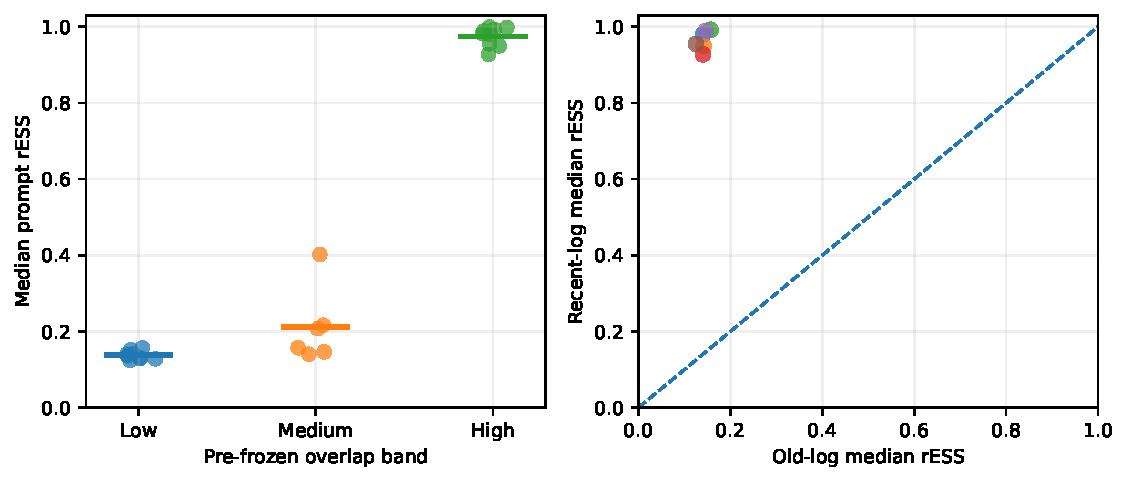
\includegraphics[width=.90\linewidth]{Figure6_svamp_external_transfer.pdf}
\caption{Frozen SVAMP transfer. Left: median prompt rESS for all 24 frozen cases grouped by the predeclared low/medium/high overlap bands; horizontal segments mark band means. Right: old-log versus recent-log median rESS for the six same-target matched comparisons present in the frozen registry. No pair reselection or gate refitting uses SVAMP outcomes.}
\label{fig:svamp}
\end{figure}

Ordinary IS remains a useful benchmark in the external layer. Across the 24 frozen SVAMP cases, its MAE and RMSE against the finite reference are \SvISMAE\ and \SvISRMSE, versus \SvPWISMAE\ and \SvPWISRMSE\ for prompt-WIS. This does not change the estimand-based reason for using prompt-WIS as primary; detailed estimator and pair-level external results are retained in Appendix~\ref{app:empirical}.

\subsection{Exploratory reward-stratum mechanism analysis}
The post-hoc analysis tests whether the binary-stratum decomposition is merely formal or illuminates the observed refresh pattern. The target references in the matched GSM8K cases lie well below $1/2$: \AlphaDevVMin--\AlphaDevVMax\ on development and \AlphaTestVMin--\AlphaTestVMax\ on the official test. Therefore $\partial m_2/\partial\alpha>0$ under the plug-in target value, so a decrease in $\widehat\alpha$ is the locally favorable direction at fixed overlap.

That favorable movement is not what dominates the data. Mean $\widehat\alpha$ changes from \AlphaDevOldAlpha\ to \AlphaDevRecentAlpha\ on development and from \AlphaTestOldAlpha\ to \AlphaTestRecentAlpha\ on the official test. Only \AlphaDevAlphaFav\ development pairs and \AlphaTestAlphaFav\ test pairs move in the favorable $\alpha$ direction. Mean $\widehat A^{\mathrm{proxy}}$ likewise rises slightly. Nevertheless, the pair-level arithmetic mean of the direct empirical $\widehat m_2^{\mathrm{proxy}}$ moment decreases after refresh in \AlphaDevMtwoFav\ development comparisons and \AlphaTestMtwoFav\ test comparisons. The mean recent/old aggregate ratios are \AlphaDevMeanMtwoRatio\ and \AlphaTestMeanMtwoRatio, respectively.

This pattern is consistent with an ``overlap-dominant'' mechanism: the strong restoration visible in empirical rESS more than offsets adverse reward-stratum movement at the aggregate empirical moment level. It should not be read as confirmatory validation of Proposition 4. The analysis was proposed after the official-test results were inspected; it uses an aggregate finite reference $V$ in place of latent prompt-specific $v_i$; and finite-$K$ plug-in moments should not be identified with their population counterparts. Its value is explanatory rather than certifying.

\begin{table}[H]
\centering
\caption{Post-hoc GSM8K mechanism analysis. Development is the primary exploratory layer; official test is exploratory replication. The publication-facing risk proxy uses the arithmetic mean of promptwise empirical $m_2$ moments, consistent with the prompt-average geometry of Corollary 2.}
\label{tab:alpha}
\small
\begin{tabular}{@{}lrr@{}}
\toprule
Quantity & Development & Official test \\
\midrule
Matched pairs & \AlphaDevPairs & \AlphaTestPairs \\
Mean rESS, old $\to$ recent & $\AlphaDevOldRess\to\AlphaDevRecentRess$ & $\AlphaTestOldRess\to\AlphaTestRecentRess$ \\
Mean $\widehat\alpha$, old $\to$ recent & $\AlphaDevOldAlpha\to\AlphaDevRecentAlpha$ & $\AlphaTestOldAlpha\to\AlphaTestRecentAlpha$ \\
Pairs with favorable $\widehat\alpha$ movement & \AlphaDevAlphaFav & \AlphaTestAlphaFav \\
Mean $\widehat A^{\mathrm{proxy}}$, old $\to$ recent & $\AlphaDevOldA\to\AlphaDevRecentA$ & $\AlphaTestOldA\to\AlphaTestRecentA$ \\
Aggregate $\widehat m_2^{\mathrm{proxy}}$ improved & \AlphaDevMtwoFav & \AlphaTestMtwoFav \\
Mean aggregate ratio, recent/old & \AlphaDevMeanMtwoRatio & \AlphaTestMeanMtwoRatio \\
\bottomrule
\end{tabular}
\end{table}

\section{Discussion}
The completed evidence now supports a three-layer interpretation rather than a single ``freshness'' story.

\paragraph{Historical evidence ages structurally.}
The fixed GSM8K frontier shows that a step-0 archive loses sequence support as the target policy evolves, while the frozen SVAMP experiment shows that the same predeclared overlap structure survives a prompt-distribution shift. The important transfer result is not that every discrepancy is numerically identical across datasets; it is that the high/medium/low evidence ordering remains visible and recent behavior again restores near-on-policy overlap. This is the empirical counterpart of the second-moment coordinate $\kappa_2$, without equating finite-sample median rESS with population $1/\kappa_2$.

\paragraph{Refresh is a two-channel operation.}
Corollary 3 separates leading risk into overlap and reward-stratum allocation. The post-hoc analysis makes that distinction empirically useful: $\widehat\alpha$ moves in the favorable direction in only a minority of matched pairs, yet the direct aggregate empirical $m_2$ proxy improves in every development and test comparison. Thus the observed refresh effect is not evidence that all risk components move together. Rather, support restoration is sufficiently strong in these runs to dominate a modest adverse shift in reward-stratum allocation. This also explains why it would be incorrect to elevate a weight-only diagnostic into an estimator-specific theorem.

\paragraph{Finite references remain measurement devices, not truth.}
The shared-reference identity shows why a common independently generated reference is especially useful for comparing old and recent logs: reference variance cancels in the expected squared-discrepancy difference. It does not make the realized reference exact. This distinction remains essential in both GSM8K and SVAMP, where one matched comparison can show worse realized absolute discrepancy even when the broader risk structure improves.

\paragraph{Diagnostics are not certificates.}
The gate results are the strongest operational negative finding. A frozen scalar rESS threshold accepts all official GSM8K test cases and all SVAMP cases; at the strict 1\% tolerance, false-accept fractions are 15.2\% and 25.0\%, respectively. The external failure therefore rules out a convenient but unsupported interpretation in which one global rESS cutoff certifies discrepancy safety across prompt distributions. Overlap remains informative---indeed the external band ordering is strong---but a deployable reuse rule must also account for reward alignment, finite-sample uncertainty, and the precision of the reference or other validation signal.

\paragraph{Estimator choice and evidence geometry.}
Prompt normalization matches the prompt-grouped estimand but introduces finite-sample self-normalization bias. Ordinary IS has smaller discrepancy in the fixed-log GSM8K benchmark and in the aggregate SVAMP benchmark, while prompt-WIS has narrower intervals in the official GSM8K analysis. This is not an inconsistency: the estimators occupy different bias--dispersion trade-offs. The main scientific conclusion---stale support deteriorates and matched refresh restores it---does not depend on claiming finite-sample dominance of prompt-WIS.

Taken together, the study suggests a practical evidence-management view of LLM reinforcement learning. A historical trace archive should not be treated as a timeless dataset. Its value is target-dependent and can be audited through exact rescoring, matched refresh, overlap diagnostics, reward-aware moments, and explicit chronological validation. When the evidence becomes weak, refreshing behavior traces is a statistically interpretable intervention rather than an arbitrary heuristic.

\section{Limitations}
The external SVAMP experiment extends the evidence across prompt distributions, but not across model scales, training algorithms, reward types, or independently trained task-specific policies. The study still uses one small instruction-tuned model, one GRPO configuration, three training seeds, and mathematics reasoning with binary correctness rewards. SVAMP reuses the same learned GRPO checkpoints; it tests prompt-distribution transfer of the reuse mechanism, not generalization to a separately trained model family or a new RL objective.

The on-policy reference is finite Monte Carlo evidence. GSM8K official test uses eight reference completions per prompt; SVAMP uses eight at ordinary targets and 32 at predeclared audit targets. Reference noise remains part of every reported OPE-reference discrepancy. Lemma 1 protects the expected squared old-versus-recent comparison from a common independent reference-variance term, but it does not turn the reference into exact policy value or guarantee realized absolute-discrepancy ordering.

Checkpoint summaries within one training seed are dependent observations from the same learning path. Pooled correlations and matched-pair counts are therefore primarily descriptive; the three independently trained seeds provide the more meaningful path-level replication. The SVAMP pair registry is deliberately sparse: it is designed as a frozen stress test, not a full second frontier. Its success supports transfer of the selected structural contrasts but does not identify every possible dataset-by-checkpoint interaction.

The theoretical contribution is intentionally narrower than a new generic SNIS theory. Proposition 1 and Theorem 1 are established importance-sampling results specialized to the sequence-level setting; Proposition 2 reorganizes the standard asymptotic variance into overlap and reward-residual components. Proposition 3 is an exact tower-property recursion for autoregressive second moments, not a generic R\'enyi chain rule. The binary-stratum result exploits the correctness-reward structure, and Lemma 1 exploits the matched shared-reference design. The present experiments do not estimate the full-vocabulary conditional $d_{2,t}$ terms in Proposition 3; sampled-token KL diagnostics should not be interpreted as those conditional R\'enyi-2 divergences.

The $\widehat\alpha$ analysis is explicitly post-hoc. It uses aggregate finite target reference $V$ inside $A^{\mathrm{proxy}}$, rather than the unobserved prompt-specific $v_i$, and therefore provides a mechanism diagnostic rather than a consistent promptwise plug-in estimator of the theoretical coefficient. The fact that its aggregate empirical moment improves in every matched comparison is useful evidence, but it should not be converted into a confirmatory guarantee or used to refit the frozen gate after the fact.

Finally, the official-test compute grid is smaller than the originally frozen pair registry. The reduction was selected from development-only computational benchmarks before official-test OPE outcomes were inspected, and the later nine-pair repair was structural rather than outcome-selected. The external FP32 repair was also made before any SVAMP OPE or reference outcomes were generated. These safeguards reduce researcher degrees of freedom but do not eliminate the need for independent replication.

\section{Conclusion}
Historical GRPO traces can remain useful after the policy that generated them has changed, but their value depends on temporal drift, overlap, reward-residual structure, and finite measurement. Along three training paths, a fixed step-0 log loses sequence support as the target checkpoint moves away. Replacing the stale log with a recent behavior log restores median prompt rESS in every matched official-test comparison and lowers mean absolute discrepancy from the shared finite on-policy reference by about 72\%, with lower discrepancy in 8 of 9 cases.

A frozen SVAMP stress test strengthens this conclusion without changing the protocol. Predeclared low/medium/high overlap ordering is preserved. Matched refresh raises mean median rESS from \SvOldRess\ to \SvRecentRess\ in \SvMatchedRessCount\ comparisons, while mean absolute reference discrepancy falls by \SvMAEReduction. The frozen scalar gate, however, accepts every external case and false-accepts \SvGateFAOne\ at the 1\% tolerance. Mechanism transfer and decision-rule transfer therefore separate cleanly.

The theory explains why. Autoregressive second-moment mismatch accumulates under a squared-weight tilted prefix law; leading SNIS risk separates into overlap and reward-residual alignment; binary correctness exposes the allocation of squared weight across reward strata; and a shared finite reference contributes the same variance term to both sides of an expected squared matched comparison. The exploratory $\widehat\alpha$ analysis further suggests that strong overlap restoration can dominate adverse reward-stratum movement rather than requiring every component to improve together.

In this setting, historical reasoning traces are reusable evaluation assets, but their reuse should be justified by the current evidence rather than checkpoint age or a single ESS threshold. The next step toward a general theory is not another universal cutoff; it is a richer, uncertainty-aware evidence manager that decides when historical traces are adequate, when they should be refreshed, and when new on-policy evidence is required.

\section*{Data and Code Availability}
The experiment is organized around frozen configuration files, pair registries, amendment manifests, identity checks, machine-readable result tables, and deterministic paper-output layers. The GSM8K paper layer does not call the model, refit the gate, or mutate upstream results. External SVAMP outputs are generated under the same provenance chain and incorporated only after the frozen external protocol is verified. The post-hoc $\widehat\alpha$ analysis is separately labeled exploratory and likewise makes no model calls, gate changes, or pair selections. The archival package retains source hashes and result-table hashes sufficient to reconstruct the reported numerical assets. A public repository URL can be attached at submission release without changing the numerical results.

\appendix
\section{Proofs and Theoretical Details}
\subsection{Proof of Proposition 1}
Absolute continuity gives $\E_\mu[W]=\int (\dd\pi/\dd\mu)\dd\mu=1$. By definition,
\[
D_2(\pi\Vert\mu)=\log\int\left(\frac{\dd\pi}{\dd\mu}\right)^2\dd\mu=\log\E_\mu[W^2]=\log\kappa_2.
\]
For i.i.d. $W_1,\ldots,W_K$,
\[
\widehat{\rESS}_K=\frac{(K^{-1}\sum_jW_j)^2}{K^{-1}\sum_jW_j^2}.
\]
The strong law and continuous mapping theorem give $\widehat{\rESS}_K\to1/\kappa_2$ almost surely. \qed

\subsection{Proof of Theorem 1}
Agapiou et al.~\cite{agapiou2017} give, for $|\phi|\le1$, the SNIS bounds $\E[(\widehat\pi_K(\phi)-\pi(\phi))^2]\le4\kappa_2/K$ and $|\E[\widehat\pi_K(\phi)]-\pi(\phi)|\le12\kappa_2/K$. Set $\phi=2R-1$. Normalized weights sum to one, so $\widehat\pi_K(\phi)-\pi(\phi)=2(\widehat v-v)$. Dividing the two inequalities by four and two yields the displayed constants. The minima with one follow from $\widehat v,v\in[0,1]$. \qed

\subsection{Proof of Proposition 2}
Write $\overline W_K=K^{-1}\sum_jW_j$ and $Z_K=K^{-1}\sum_jW_j(R_j-v)$. Then $\widehat v-v=Z_K/\overline W_K$. Since $\E_\mu[W]=1$, $\overline W_K\to1$ almost surely. Also $\E_\mu[W(R-v)]=0$ and $\Var_\mu\{W(R-v)\}=m_2$. The classical CLT and Slutsky's theorem give the SNIS limit. By definition of $\nu_2$, $A_\mu=m_2/\kappa_2$, so $m_2=\kappa_2A_\mu$. \qed

\subsection{Proofs of Corollaries 1 and 2}
Corollary 1 follows immediately from $m_{2,o}=\kappa_oA_o$, $m_{2,r}=\kappa_rA_r$, and $\kappa=e^{D_2}$. Taking logarithms gives the sufficient condition.

For Corollary 2, with fixed $n$, Proposition 2 supplies independent promptwise limits $\sqrt K(\widehat v_i-v_i)\Rightarrow N(0,m_{2,i})$. Joint convergence of the finite collection and linearity yield
\[
\sqrt K(\widehat V^{\pWIS}-V_n)=\frac1n\sum_i\sqrt K(\widehat v_i-v_i)
\Rightarrow N\!\left(0,\frac1{n^2}\sum_i m_{2,i}\right).
\]
\qed

\subsection{Proof of Proposition 3}
Condition on $H_{t-1}$. By the multiplicative definition of $W_t$ and the tower property,
\begin{align*}
\kappa_{2,t}
&=\E_\mu[W_{t-1}^2w_t(A_t\mid H_{t-1})^2]\\
&=\E_{\mu_{1:t-1}}\!\left[W_{t-1}^2\E_{A_t\sim\mu_t(\cdot\mid H_{t-1})}[w_t^2]\right]\\
&=\kappa_{2,t-1}\E_{\nu_{t-1}^{(2)}}[c_t(H_{t-1})].
\end{align*}
Iterating from $\kappa_{2,0}=1$ and taking logarithms gives the telescoping representation. Jensen's inequality yields the lower bound because $c_t(h)=\exp\{d_{2,t}(h)\}$. Since $c_t(h)=1+\chi^2(\pi_t(\cdot\mid h)\Vert\mu_t(\cdot\mid h))\ge1$, $\kappa_{2,t}$ is nondecreasing. Finally,
\[
\E_{\nu_{t-1}^{(2)}}[c_t]-\E_{\mu_{1:t-1}}[c_t]
=\frac{\Cov_{\mu_{1:t-1}}(W_{t-1}^2,c_t)}{\kappa_{2,t-1}}.
\]
The absorbing-EOS extension sets $w_t=c_t=1$ and $d_{2,t}=0$ after termination. \qed

\subsection{Proof of Proposition 4 and Corollary 3}
For $R\in\{0,1\}$,
\[
(R-v)^2=(1-v)^2\ind\{R=1\}+v^2\ind\{R=0\}.
\]
Multiplying by $W^2$ and taking $\mu$-expectation gives $m_2=(1-v)^2\kappa_1+v^2\kappa_0$. Since $\kappa_1=\alpha_\mu\kappa_2$ and $\kappa_0=(1-\alpha_\mu)\kappa_2$, the stated decomposition follows; differentiation gives $\partial m_2/\partial\alpha_\mu=\kappa_2(1-2v)$. Applying the same expression to old and recent behavior laws for one fixed target gives Corollary 3. \qed

\subsection{Proof of Lemma 1}
Condition on the frozen prompt set and write $\Delta_s=\widehat V_s-V_n$ and $\eta=\widehat V_{\mathrm{ref}}-V_n$. By independence and $\E[\eta\mid x_{1:n}]=0$,
\[
\E[(\Delta_s-\eta)^2\mid x_{1:n}]=\E[\Delta_s^2\mid x_{1:n}]+\E[\eta^2\mid x_{1:n}].
\]
Subtracting the expressions for $s=r$ and $s=o$ cancels the common reference-variance term. The realized identity follows by direct expansion. \qed

\subsection{Verification of Example 1}
Under either behavior law,
\[
\kappa_2=\sum_{y=1}^{3}\frac{\pi(y)^2}{\mu(y)}=\frac{10}{9}.
\]
The target value is $v=1/3$. Direct substitution into $m_2=\E_\mu[W^2(R-v)^2]$ yields $m_{2,A}=25/81$ and $m_{2,B}=16/81$. \qed

\subsection{Supplementary finite-sample bounds}
The following bounds are retained for completeness and are not used as numerical certificates.

\begin{corollary}[Supplementary grouped-prompt MSE bound]
Condition on frozen prompts and suppose historical completion groups are independent across prompts. Let $\bar\kappa_2=n^{-1}\sum_i\kappa_{2,i}$. Then
\begin{equation}
\E[(\widehat V^{\pWIS}-V_n)^2\mid x_{1:n}]
\le \min\!\left\{1,\frac{\bar\kappa_2}{nK}+\frac{36\bar\kappa_2^2}{K^2}\right\}.
\end{equation}
\end{corollary}
The first term receives the $1/n$ variance reduction from averaging independent prompt groups. The second is the squared worst-case bias upper-bound induced by the per-prompt SNIS bound; it is not an intrinsic bias floor and can be numerically vacuous at the present $K$.

\begin{proposition}[Supplementary finite-sample overlap--residual bound]
Under the assumptions of Theorem 1, let $m_2=\E_\mu[W^2(R-v)^2]$. For every $a\in(0,1)$,
\begin{equation}
\E[(\widehat v-v)^2]\le \frac{m_2}{Ka^2}+\frac{\kappa_2-1}{\kappa_2-1+K(1-a)^2}.
\end{equation}
Consequently,
\begin{equation}
\E[(\widehat v-v)^2]\le
\min\!\left\{\frac{\kappa_2}{K},\ \inf_{0<a<1}\left[\frac{m_2}{Ka^2}+\frac{\kappa_2-1}{\kappa_2-1+K(1-a)^2}\right],\ 1\right\}.
\end{equation}
\end{proposition}
The proof splits on $\overline W_K\ge a$, applies $\E Z_K^2=m_2/K$ on that event, and controls $\Pr(\overline W_K<a)$ with Cantelli's one-sided inequality using $\Var(\overline W_K)=(\kappa_2-1)/K$.

\section{Additional Empirical Summaries}
\label{app:empirical}
\begin{table}[H]
\centering
\caption{Fixed-log Spearman correlations for prompt-WIS. Target-step association with rESS is strong; association between rESS and realized reference discrepancy is weaker and path-dependent.}
\small
\begin{tabular}{@{}llrr@{}}
\toprule
Split & Seed & Target step vs. rESS & rESS vs. abs. discrepancy \\
\midrule
Development & 20260826 & $-0.908$ & $-0.598$ \\
Development & 20260827 & $-0.854$ & $-0.128$ \\
Development & 20260828 & $-0.605$ & $+0.239$ \\
Development & pooled & $-0.745$ & $-0.316$ \\
Official test & 20260826 & $-0.881$ & $-0.048$ \\
Official test & 20260827 & $-0.905$ & $-0.595$ \\
Official test & 20260828 & $-0.548$ & $-0.095$ \\
Official test & pooled & $-0.767$ & $-0.098$ \\
\bottomrule
\end{tabular}
\end{table}

\begin{table}[H]
\centering
\caption{Matched refresh results by training seed. Mean reduction is $1-$ recent absolute discrepancy / old absolute discrepancy.}
\small
\begin{tabular}{@{}llrrrr@{}}
\toprule
Split & Seed & Improved & Mean old & Mean recent & Mean reduction \\
\midrule
Development & 20260826 & 10/15 & 0.003450 & 0.001597 & 53.7\% \\
Development & 20260827 & 9/15 & 0.002113 & 0.001752 & 17.1\% \\
Development & 20260828 & 15/15 & 0.009480 & 0.001634 & 82.8\% \\
Official test & 20260826 & 2/3 & 0.001392 & 0.001132 & 18.7\% \\
Official test & 20260827 & 3/3 & 0.011081 & 0.001104 & 90.0\% \\
Official test & 20260828 & 3/3 & 0.005127 & 0.002692 & 47.5\% \\
\bottomrule
\end{tabular}
\end{table}

\begin{table}[H]
\centering
\caption{Observed fixed-log tolerance horizon on the reduced official-test grid. Entries are descriptive of this grid, not universal time horizons.}
\small
\begin{tabular}{@{}lrrrr@{}}
\toprule
Seed & $\varepsilon=0.01$ & $\varepsilon=0.02$ & $\varepsilon=0.05$ & Targets within 1\% \\
\midrule
20260826 & 400 & 400 & 400 & 8/8 \\
20260827 & 160 & 400 & 400 & 3/8 \\
20260828 & 400 & 400 & 400 & 8/8 \\
\bottomrule
\end{tabular}
\end{table}

\begin{table}[H]
\centering
\caption{Finite on-policy reference inclusion within the OPE bootstrap interval. These are reference-inclusion rates, not coverage probabilities.}
\small
\begin{tabular}{@{}lrr@{}}
\toprule
Split & Ordinary IS & Prompt-WIS \\
\midrule
Development & 60/60 (1.000) & 44/60 (0.733) \\
Official test & 24/24 (1.000) & 16/24 (0.667) \\
\bottomrule
\end{tabular}
\end{table}

\begin{table}[H]
\centering
\caption{SVAMP estimator benchmark over the 24 frozen representative cases. Values are discrepancies from the finite external reference.}
\small
\begin{tabular}{@{}lrr@{}}
\toprule
Estimator & Mean absolute discrepancy & RMSE \\
\midrule
Ordinary IS & \SvISMAE & \SvISRMSE \\
Prompt-WIS & \SvPWISMAE & \SvPWISRMSE \\
\bottomrule
\end{tabular}
\end{table}

\paragraph{External pair-level audit.}
The frozen SVAMP registry contains 24 pair-seed cases (eight representative pair definitions across three seeds): nine low-overlap, six medium-overlap, and nine high-overlap cases. All three seed-level band means preserve high $>$ medium $>$ low. Detailed pair-level values, bootstrap intervals, gate decisions, and diagnostics are retained in the machine-readable T08 table rather than reproduced as a 24-row typeset table here.

\paragraph{Exploratory mechanism audit.}
The post-hoc program analyzes 54 pre-existing matched comparisons (45 development and 9 test) and validates raw recomputed median rESS against the frozen T04 matched-comparison table before accepting mechanism outputs. Its manifest labels the research status \emph{exploratory/post-hoc}; it calls no model, uses no CUDA, refits no gate, selects no new pairs, and mutates no upstream results.

\section{Protocol Amendments and Reproducibility Audit}
\label{app:protocol}
The numerical analysis was designed to preserve chronological separation among development, official-test, external, and exploratory evidence.

\paragraph{Canonical GSM8K rescoring.}
An identity audit detected a small discrepancy between generation-time behavior log probabilities and a separately evaluated teacher-forced path. Before non-identity formal OPE pairs were evaluated, the denominator and numerator of the formal sequence ratio were both moved to symmetric canonical FP32 teacher forcing. Generation-time probabilities were retained as immutable audit evidence. This changed the numerical scoring path, not sampled trajectories, rewards, training checkpoints, or target definitions.

\paragraph{Official-test pair-grid reduction and structural repair.}
The original test registry contained 117 behavior-target pairs. Before inspecting official-test OPE outcomes, development-only computational benchmarks selected the smallest reduced grid meeting pre-specified distortion criteria, initially 36 pairs. During official-test analysis, a structural dependency in the rolling contrast was identified: every retained rolling pair requires the corresponding step-0 fixed comparator at the same target. Exactly nine such pairs were added. The repair did not select pairs by observed errors or rewards.

\paragraph{Official-test reference size.}
A development-only sample-size benchmark performed before official-test outcomes showed that eight samples per prompt met the predeclared distortion checks for the reduced test grid. The official-test reference generation therefore used eight samples for both main and audit targets under a recorded amendment. Historical behavior $K=16$, estimators, bootstrap rule, gate diagnostic, and gate tolerances were unchanged.

\paragraph{SVAMP precision-contract repair.}
Before any SVAMP OPE or reference outcomes were generated, an implementation audit identified a mismatch between the inherited generation/scoring precision contract and the main experiment's canonical FP32 contract. The corrected Program 08 run uses FP32 policy inference and symmetric FP32 teacher-forced scoring. Superseded lower-precision external assets are not used for results. The Program 08 manifest records 1,000 prompts, eight representative pairs per seed, $K=16$, $L=8$ at main targets and $L=32$ at predeclared audit steps, as well as the frozen-gate and pair-registry hashes.

\paragraph{Deterministic paper and exploratory layers.}
Program 09 is CPU-only and deterministically converts machine-readable upstream results into paper tables, figures, values, and a provenance manifest; it does not call the model, refit the gate, or mutate upstream results. The external T08 file is hash-verified against the Program 08 manifest before inclusion. The post-hoc $\widehat\alpha$ program is separately versioned and likewise reads immutable rescore artifacts without model calls. Its v2 aggregation contract states that the publication-facing prompt-average risk proxy uses the arithmetic mean of promptwise $m_2$ proxies; promptwise geometric ratios are retained only as heterogeneity diagnostics.

The frozen gate SHA-256 is
\begin{center}\ttfamily\small
37c810f9c2c05b617e69dfe0b3b43561b791c1596ebce2c0fbc0f3566357f136.
\end{center}
The protocol configuration hash is
\begin{center}\ttfamily\small
2a4934d6036e5bc87e629dd2883dc7c38d65e0b98ad6bc248bec077ae654ecc8.
\end{center}
The final Program 08 T08 hash recorded in its manifest is
\begin{center}\ttfamily\small
f7c90c506008ba8c167be8f131b208a467ff905891f0118792eac52a6de7cfd8.
\end{center}
These identifiers make the manuscript auditable before a public repository URL is assigned.

\begin{thebibliography}{99}
\bibitem{shao2024deepseekmath} Z. Shao et al. DeepSeekMath: Pushing the Limits of Mathematical Reasoning in Open Language Models. arXiv:2402.03300, 2024.
\bibitem{deepseek2025r1} DeepSeek-AI et al. DeepSeek-R1: Incentivizing Reasoning Capability in LLMs via Reinforcement Learning. arXiv:2501.12948, 2025.
\bibitem{dudik2011dr} M. Dud\'ik, J. Langford, and L. Li. Doubly Robust Policy Evaluation and Learning. ICML, 2011.
\bibitem{jiang2016dr} N. Jiang and L. Li. Doubly Robust Off-policy Value Evaluation for Reinforcement Learning. ICML, 2016.
\bibitem{swaminathan2015selfnorm} A. Swaminathan and T. Joachims. The Self-Normalized Estimator for Counterfactual Learning. NeurIPS, 2015.
\bibitem{thomas2015hcpi} P. Thomas, G. Theocharous, and M. Ghavamzadeh. High Confidence Policy Improvement. ICML, 2015.
\bibitem{kuzborskij2021confident} I. Kuzborskij, C. Vernade, A. Gy\"orgy, and C. Szepesv\'ari. Confident Off-Policy Evaluation and Selection through Self-Normalized Importance Weighting. AISTATS, 2021.
\bibitem{liu2020horizon} Y. Liu, P.-L. Bacon, and E. Brunskill. Understanding the Curse of Horizon in Off-Policy Evaluation via Conditional Importance Sampling. ICML, 2020.
\bibitem{bhargava2024ope} A. Bhargava, L. Jain, B. Kveton, G. Liu, and S. Mukherjee. Off-Policy Evaluation from Logged Human Feedback. arXiv:2406.10030, 2024.
\bibitem{zheng2025gspo} C. Zheng et al. Group Sequence Policy Optimization. arXiv:2507.18071, 2025.
\bibitem{leroux2025topr} N. Le Roux et al. Tapered Off-Policy REINFORCE: Stable and Efficient Reinforcement Learning for LLMs. arXiv:2503.14286, 2025.
\bibitem{ackermann2025ocrm} J. Ackermann, T. Ishida, and M. Sugiyama. Off-Policy Corrected Reward Modeling for Reinforcement Learning from Human Feedback. COLM, 2025; arXiv:2507.15507.
\bibitem{agapiou2017} S. Agapiou, O. Papaspiliopoulos, D. Sanz-Alonso, and A. M. Stuart. Importance Sampling: Intrinsic Dimension and Computational Cost. Statistical Science, 32(3):405--431, 2017.
\bibitem{martino2017ess} L. Martino, V. Elvira, and F. Louzada. Effective Sample Size for Importance Sampling Based on Discrepancy Measures. Signal Processing, 131:386--401, 2017.
\bibitem{cardoso2022brsnis} G. Cardoso, S. Samsonov, A. Thin, E. Moulines, and J. Olsson. BR-SNIS: Bias Reduced Self-Normalized Importance Sampling. NeurIPS, 2022.
\bibitem{li2025repo} S. Li, Z. Zhou, W. Lam, C. Yang, and C. Lu. RePO: Replay-Enhanced Policy Optimization. arXiv:2506.09340, 2025.
\bibitem{mroueh2025grpo} Y. Mroueh et al. Revisiting Group Relative Policy Optimization: Insights into On-Policy and Off-Policy Training. arXiv:2505.22257, 2025.
\bibitem{tian2026mugrpo} M. Tian, Y. Xie, and C. Wei. How Off-Policy Can GRPO Be? Mu-GRPO for Efficient LLM Reinforcement Learning. arXiv:2605.17570, 2026.
\bibitem{elvira2022ess} V. Elvira, L. Martino, and C. P. Robert. Rethinking the Effective Sample Size. International Statistical Review, 90(3):525--550, 2022.
\end{thebibliography}

\end{document}
